\documentclass[9pt,aspectratio=169]{beamer}

\usepackage{nicefrac}
\usepackage{tabularx}
\usepackage{xcolor}
\newcolumntype{Y}{>{\centering\arraybackslash\leavevmode}X}
\renewcommand\tabularxcolumn[1]{m{#1}}% for vertical centering text in X column
\usepackage{luamplib}
  \mplibsetformat{metafun}
  \mplibtextextlabel{enable}
\everymplib{input mpcolornames; input repere; input macros; beginfig(1);}
\everyendmplib{endfig;}

\usetheme{graham}

\title{Geometry Probability}
\subtitle[Graham Middle School]{Graham Middle School Math Olympiad Team}

\begin{document}
\maketitle

\begin{frame}{GEOMETRIC PROBABILITY}
  \begin{columns}[T]
    \begin{column}{0.5\textwidth}
      In the probability unit, we learned that the probability of a certain outcome was defined as the number of desired outcomes divided by the total number of possible outcomes.
      
      Using combinatorics, we could count the different outcomes to calculate this ratio.
      
      Probability can also be defined geometrically, most often in terms of area.  In this case, the probability is the area of the desired region divided by the total area.  Consider the following example:

    \end{column}
    \begin{column}{0.5\textwidth}
      \begin{problem}
        What is the probability of a dart randomly dropped onto a dartboard hitting the bullseye, if the diameter of the board is $50$ cm, and the diameter of the bullseye is 1 cm?
      \end{problem}
      \begin{center}
        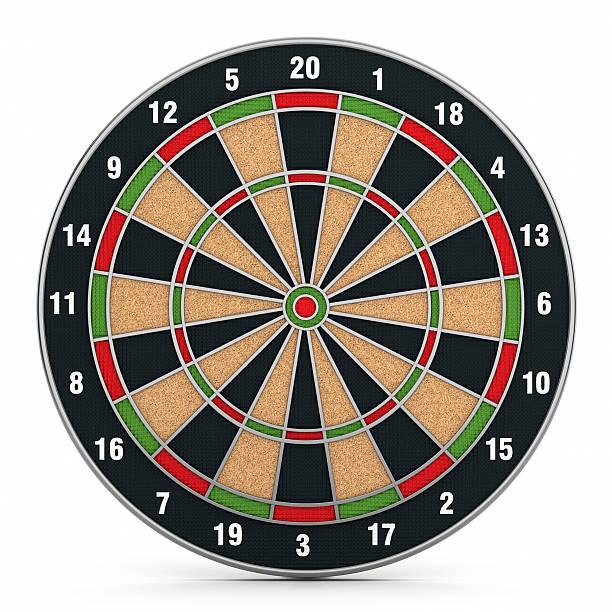
\includegraphics[width=0.4\textwidth]{16 - Geometric Probability/darts.png}
      \end{center}
      The area of the entire board is $(\pi 25)^2$, while the area of the bullseye is $\left(\dfrac{\pi}{2}\right)^2$.  The probability is the ratio of these two areas, which is $\dfrac{1}{2500}$.

    \end{column}
  \end{columns}
\end{frame}

\begin{frame}{1-DIMENSIONAL PROBABILITY}
  \begin{columns}[T]
    \begin{column}{0.5\textwidth}
      Sometimes geometric probability questions can occur in 1-dimensional scenarios.  In that case, the probability is the ratio of the desired length to the entire possible length.  The example below is an illustration of such a situation.
      \begin{problem}
        A satellite is in orbiting the earth along the planet’s equator.  The retro thrusters accidentally fire, and the orbit decays, meaning the satellite will randomly land at some point along the earth’s equator.  What is the probability that it will crash on dry land?
      \end{problem}
      The denominator is the circumference of the earth along its equator.  The numerator can be estimated as the widths of South America and Africa where the equator crosses those two continents.  When you measure those values on a globe or map, the probability of crashing on dry land is rather small.
    \end{column}
    \begin{column}{0.5\textwidth}
      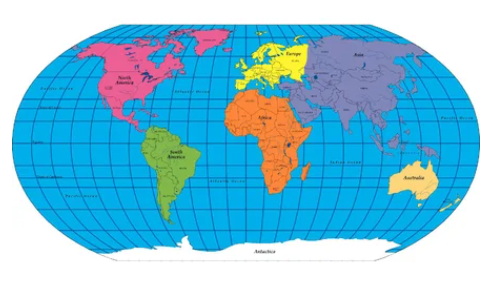
\includegraphics[width=\textwidth]{16 - Geometric Probability/map.png}
    \end{column}
  \end{columns}
\end{frame}

\begin{frame}{3-DIMENSIONAL PROBABILITY}
  \begin{columns}[T]
    \begin{column}{0.5\textwidth}
      If the problem is 3-dimensional, then the probability is calculated as the volume of the desired region, divided by the entire possible volume.  Consider the following illustrative example.
      \begin{problem}
        Gas molecules are moving randomly inside a spherical glass bulb.  If the diameter of the bulb is $20$ cm, what is the probability that a gas molecule is located within 1 cm of the glass? 
      \end{problem}
      The probability is simply the volume within $1$ cm of the edge of the sphere divided by the total volume of the sphere.  The total volume of the sphere is $(\dfrac{4}{3}\pi10)^3 = \dfrac{4000\pi}{3}$.  The volume with $1$ cm of the edge is the volume of a $10$ cm radius sphere minus the volume of a $9$ cm radius sphere. This is 
      \[\frac{(4000 - 2916)\pi}{3} = \frac{1084\pi}{3}.\]  The probability is therefore $\dfrac{1084}{4000} = \dfrac{271}{1000}$.

    \end{column}
    \begin{column}{0.5\textwidth}
      % TODO illustration
    \end{column}
  \end{columns}
\end{frame}

\begin{frame}{ANGULAR PROBABILITY}
  \begin{columns}[T]
    \begin{column}{0.5\textwidth}
      Sometimes it is easiest to solve a probability problem in terms of the allowed range of angles divided by the total possible range of angles.  In this way, a 2-dimensional area problem can often be simplified into a one dimensional angular calculation.  Consider the illustrative example below.
      \begin{center}
        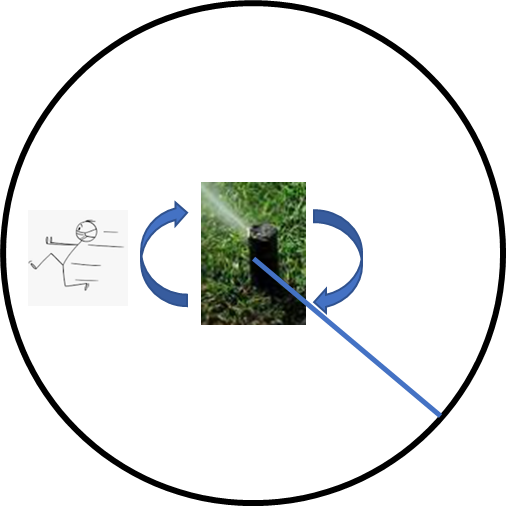
\includegraphics[width=0.6\textwidth]{16 - Geometric Probability/sprinkler.png}
      \end{center}
    \end{column}
    \begin{column}{0.5\textwidth}
      \begin{problem}
        A sprinkler pops up on the lawn with its nozzle pointed at a random angle relative to your location.  It then rotates at a speed of $2$ rpm.  When you hear the sprinkler pop up, you immediately run away from the sprinkler.  If it takes you $10$ seconds to run out of range of the spray, what is the probability that you will get wet?
      \end{problem}
      The initial direction of the sprinkler is random, and you run directly away from the sprinkler, not taking into account if the spray is rotating towards or away from you.  At a rotational rate of $2$ rpm, the sprinkler covers $360°$ in $30$ sec. In $10$ sec. it will traverse $120°$, so the probability that you get wet is $\dfrac{120}{360} = \dfrac{1}{3}$.

    \end{column}
  \end{columns}
\end{frame}

\begin{frame}{Exercises}
  \begin{columns}[T]
    \begin{column}{0.5\textwidth}
      \begin{enumerate}
        \item A point $P$ is randomly placed inside of a square.  A circle is inscribed inside of the same square.  What is the probability that $P$ is located inside of the circle? 
        \item A camera is randomly triggered to take a photo of a standard clockface.  What is the probability that the minute hand is pointed between the $5$ o’clock and $7$ o’clock positions?
        \item An inverted (point is at the bottom) cone is filled with sand.  Mixed in with the sand is one special grain made of diamond. If the cone has height h, what is the probability that the grain is located below the midpoint of the height?
        \item An isosceles right triangle has a point $P$ located randomly along its perimeter.  What is the probability that the point can be found on the hypotenuse?
        \seti
      \end{enumerate}
    \end{column}
    \begin{column}{0.5\textwidth}
      \vspace*{-2.6em}
      \begin{enumerate}
        \conti
        \item A trapezoid with a lower base of $10$ and an top length of 4 has a height of 6.  We draw a line parallel to the base that creates two trapezoids, each with a height of 3.  If a point is located randomly within the initial trapezoid, what is the probability that it can be found in the upper trapezoid after the demarcation line is drawn?
        \item A right circular cone has a height of $12$ and base with radius $5$.  What is the probability that a point located randomly on the surface of this cone can be found on the base?
        \item A circle is inscribed a triangle with side lengths $8$, $15$, and $17$.  What is the probability that a point randomly located within the triangle can be found outside of the circle?
        \item A meter stick is marked in centimeter increments, with each $100$ integer lengths labeled.  What is probability that a point randomly located on the meter stick is within $1$ cm of a mark whose value is the cube of an integer?        
      \end{enumerate}
    \end{column}
  \end{columns}
\end{frame}

\begin{frame}{Challenge problems}
  \begin{columns}[T]
    \begin{column}{0.5\textwidth}
      \begin{enumerate}
        \item Let $C$ be a circle with radius $4$.  Points $A$ and $B$ are chosen at random on the circumference of $C$.  What is the probability that $AB \leq 4\sqrt{3}$? Express in the form $m/n$, where $m$ and $n$ are relatively prime positive integers.

        \item Right triangle $ABC$ with $\angle BCA$ as its right angle has $m\angle ABC = 60°$, and $AB = 10$.  Let $P$ be randomly chosen inside $\triangle ABC$ and extend segment $BP$ to meet segment $AC$ at $D$.  What is the probability that $BD > 5\sqrt{2}$? 
        \seti
      \end{enumerate}
    \end{column}
    \begin{column}{0.5\textwidth}
      \begin{enumerate}
        \conti
        \item $x$ and $y$ are two positive real numbers chosen randomly and uniformly in the interval $[0,\ 2].$  In other words, the possible area is a square $2$ units on a side in the Cartesian Plane where $x$ and $y$ are both positive.  What is the probability that $x^2 + y^2 \geq 1$ and $y \geq x?$  Hint, what shape is defined by the curve $x^2 + y^2 = 1$?

        \item The circle with center at point $O$ has a diameter of $10$.  Point $P$ is randomly placed along the diameter $AB$.  If diameter $AB$ bisects chord $CD$ at point $P$, what is the probability that $CP \geq 3$?
        
      \end{enumerate}
    \end{column}
  \end{columns}
\end{frame}


% \begin{frame}{Title}
%   \begin{columns}[T]
%     \begin{column}{0.5\textwidth}
%     \end{column}
%     \begin{column}{0.5\textwidth}
%     \end{column}
%   \end{columns}
% \end{frame}

\end{document}
